%************************************************
\chapter{Implementation and evaluation}
\label{cap:implementation}
%************************************************

In this chapter the architecture of the whole system is explained as long as
the motivation that led us to these choices.

%% TODO ???
When chosing a suitable backend for our System we needed to take care of all the
features it must be able to perform (see \autoref{tab:matrix}). Without all these
needs fullfilled the System cannot bring any original contributions.

\section{Architecture}
\label{sec:implementation:arch}

The architecture is divided in two main parts, the task creation (managed by
the \hyperref[sec:configurator]{Configurator}) and the task execution (managed by
the \hyperref[sec:exec-layer]{Execution layer}).
As shown in \autoref{fig:architecture2} in the \hyperref[cap:model]{Model}
this two parts can be safely separated into standalone components.

\subsection{Configurator}
\begin{figure}[htb]
    \centering
    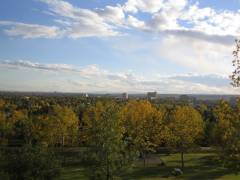
\includegraphics[width=\columnwidth]{crowdsearcher}
    \caption{The Crowdsearcher interface.}
    \label{fig:crowdsearcher}
\end{figure}
The configuration and the management of the Task/Work lifecycle is demanded to a
third part component, the \textbf{CrowdSearcher}. As descibed in
\ref{sec:bg:crowdsearch} the \emph{CrowdSearcher} is a \emph{centralized} human
computation platform able to execute the task once the user reached the
\emph{CrowdSearcher} website. For the execution the \emph{CrowdSearcher} give its
default implementation for the most common Task.

% TODO cos'è
The \emph{CrowdSearcher} has been implemented using the
\href{http://www.webratio.com}{WebRatio} tool and so is a Java standard
web-application.


\subsection{Execution Layer}
\begin{figure}[htb]
    \centering
    
\includegraphics[width=0.6\columnwidth]{nodejs}
    \caption{Official NodeJS logo.}
    \label{fig:node-logo}
\end{figure}
The execution layer is being developed using the great flexibility of \citetitle{node}.
Node.js is a platform built on Chrome's JavaScript runtime for easily building fast,
scalable network applications. Node.js uses an event-driven, non-blocking I/O model
that makes it lightweight and efficient, perfect for data-intensive real-time
applications that run across distributed devices.
This platform was chosen due to the great speed of the request-response cycle
when dealing with relatively small files (like in our scenario).

Due to the great hype around \citetitle{node} and the ease of developing
libraries for this platform, there are thousands of these being developed and
made available via the built-in package manager (\code{npm}).\\

For the implementation of the sever we used the \citetitle{express} web
application framework. This framework allow to create easy routing on pages and
provide a robust templating system. With all these features we were able to
create a REST web-server that interact with the \emph{Configurator} in order to
recieve \utask{}, execute the code and post the results back to the Configurator.

The \emph{execution layer} allow the \utask{} implementation to inherith a
\js{} \emph{Class} that give a set of API for retrieving Task configuration,
gathering data and eventially post the \utask{} results back to the
\emph{Configurator}.\\

The storage of the \utask{} implementations is made using the filesystem because
the resources needed to execute a \utask{} are almost text or binary files like
images or \js{}/\ac{CSS} files. If for a certain task a custom default\footnote{
By default we mean a single implementation for all the platforms/devices, see
\ref{} } implementation is provided than a \code{default} folder is created for
that task containing all the files. If the \emph{Requester} provides a
platform-specific implementation than a folder with the platform name (e.g.
\code{mobile}, \code{tablet}, etc.) is created and the code qill be uploaded
there. When a user visit the page containig the logic to run a task, then according
to the strategy configured the right implementation will be sent to the device.


\section{Performance comparison???}
\label{sec:implementation:performance}

TODO ??
